\section{Commands}

Users use GMAT's command subsystem to design the mission timeline that they would like to model.
In GMAT, this timeline is called the mission control sequence.  It consists of a list of
instructions defining the time ordered sequence of actions that occur to model the mission GMAT is
simulating.

The incorporation of estimation into GMAT necessitates extension of the mission control sequence to
accommodate the instructions required to perform estimation specific tasks.  In addition, some of
the existing commands in GMAT need to be modified to neet the needs of the estimation process.

GMAT will include four new commands tailored to estimation: RunEstimator, RunSimulator, Estimate,
and EndEstimate.  The Propagate command will be extended work with the expanded capabilities of the
state vector, described earlier in this chapter, and to function correctly when included as part of
an estimation control sequence defined by the Estimate and EndEstimate commands.

Many estimation tasks can be performed through simple propagation of the estimation state vector
and related quantities, with no events or state changes dictated outside of the control provided by
the estimator.  GMAT provides two commands designed to run estimation in the mission control
sequence using this paradigm: the RunEstimator and the RunSimulator commands.  Like the
Propagate command, these commands use GMAT's propagation subsystem to perform numerical or analytic
propagation of the evolving elements of a state vector.  Figure~\ref{fig:PropEnabledCommands} shows
the highest level view of the lifetime of these commands.

\begin{figure}[htb]
\centering
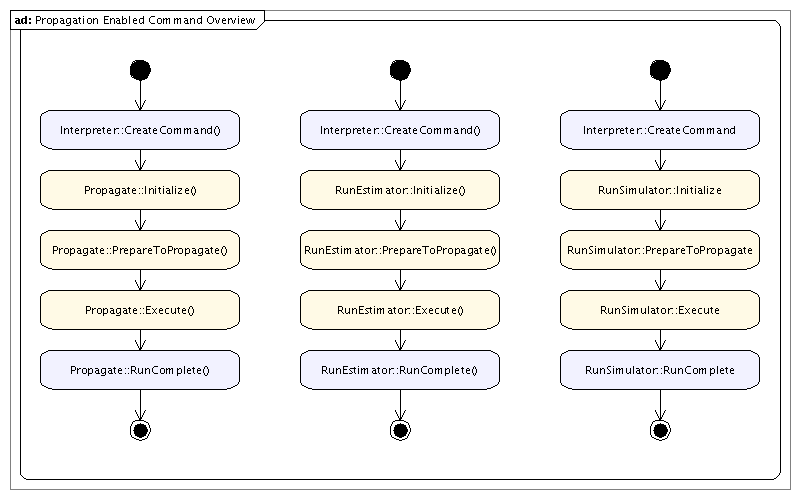
\includegraphics[400,250]{Images/PropagationEnabledCommandOverview.png}
\caption{Commands that Propagate Directly}
\label{fig:PropEnabledCommands}
\end{figure}

Each command is created as a stand alone entity by an interpreter when a script calling for the
command is opened.  When a user tells GMAT to run the script, the elements constructed by the
interpreter are passed into the Sandbox responsible for the run.  This object passing includes
insertion of the mission control sequence containing the propagation enabled command into the
Sandbox and setting of the object stores and environment data on the commands. The next call to the
command is a call to its Initialize() method, which ensures that all of the necessary elements
needed by the command exist, and sets pointers to those elements.  When the command fired in the
mission control sequence, the first phase of execution is a call to the command's
PrepareToPropagate() method, which constructs and populates the state vectors used in the execution
of the command.  Following this call, the command is executed, and runs to completion.  When the
mission control sequence has finished running, the RunComplete method is called on teh command,
completing the sequence of actions taken on the command.

The Estimate command provides a more customizable approach for users that need to include more
complicated control flow in the estimation process.  An Estimate command does not propagate
directly.  Instead, it defines the start of an estimation sequence designed to model the portion of
the mission control sequence that is being estimated.  The estimation sequence is terminated with
an EndEstimate command. Users define the timeline for the estimation process by adding commands
between teh Estimate command and the EndEstimate command.  This command pair functions similarly to
other command pairs found in GMAT: the Estimate command manages an estimator and a control
sequence, and drives the estimator state machine and control sequence in a synchronized fashion in
order to solve the estimation process.  Figure~\ref{fig:EstimateCommandOverview} shows the high
level view of the processes performed over the life of an Estimate/EndEstimate command pair.

\begin{figure}[htbp]
\centering
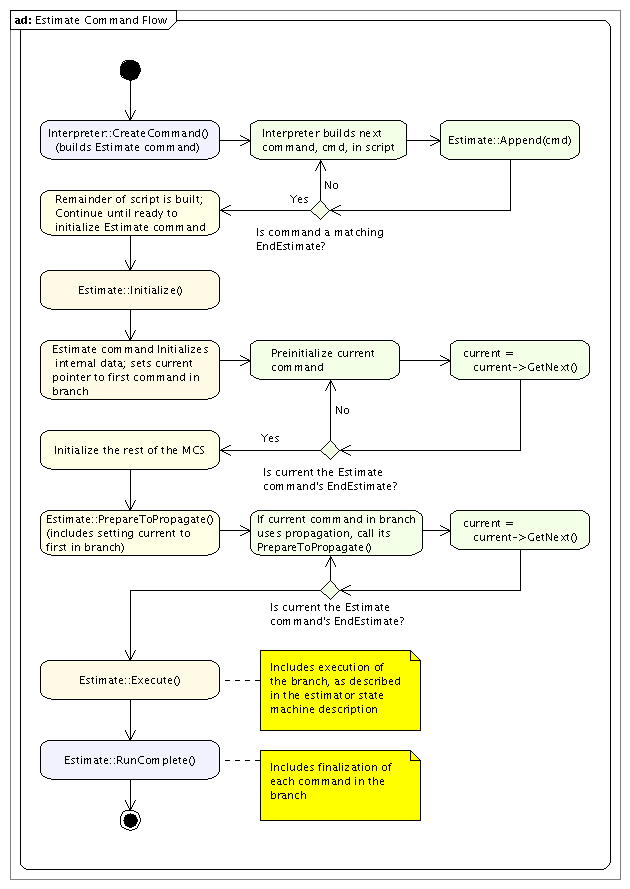
\includegraphics[315,445]{Images/EstimateCommandFlow.png}
\caption{Estimation with an Estimation Control Sequence}
\label{fig:EstimateCommandOverview}
\end{figure}



\subsection{Estimation Commands that Propagate}

\subsubsection{RunEstimator}

\subsubsection{RunSimulator}



\subsection{Estimate and EndEstimate}

\subsection{Propagate}

The Propagate command is used to control both fine grained and large scale evolution of mission
elements in GMAT.